\documentclass{article}

\author{Tran Van Tan Khoi}

\date{May 22, 2025}

\title{Weekly Homework Report \#8}

\usepackage[utf8]{inputenc}
\usepackage[a4paper,top=2cm,bottom=2cm,left=3cm,right=3cm,marginparwidth=1.75cm]{geometry}
\usepackage[colorlinks=true, allcolors=blue]{hyperref}
\usepackage{graphicx}

\begin{document}

\maketitle

\section{Introduction}
\label{introduction}



The source code is available on \href{https://github.com/xtrkoi/throwaway-rep}{Github}.


\begin{figure*}[h]
    \centering
    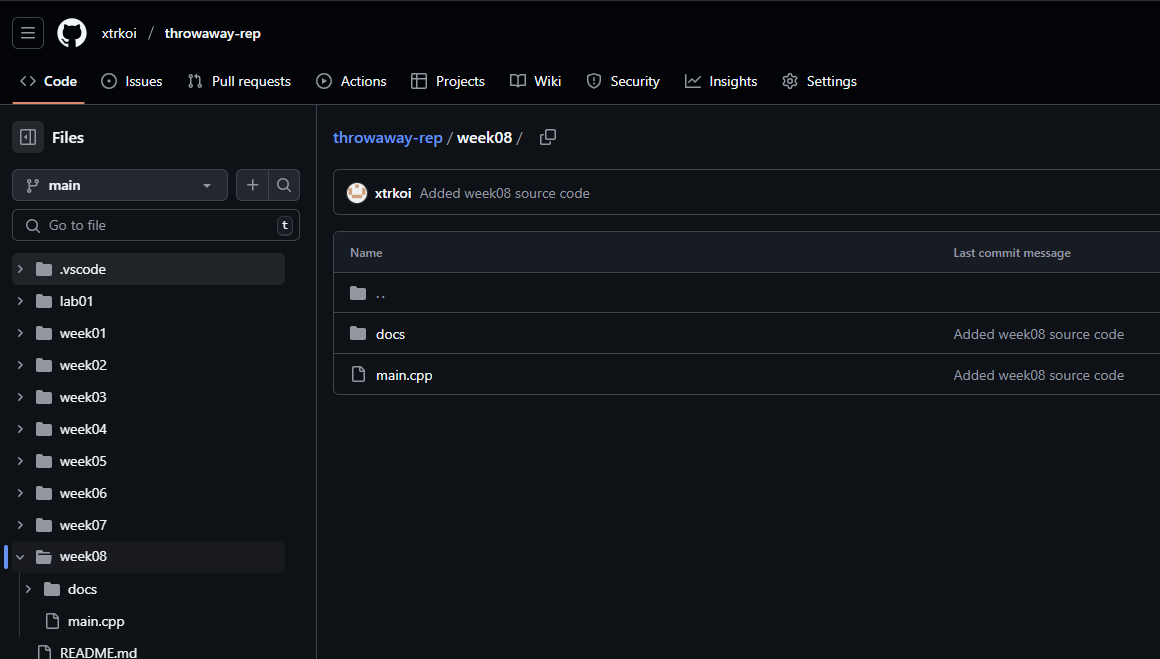
\includegraphics[width=12cm]{images/github_page.png}
\end{figure*}


\section{Graph Representation}
\label{graph_representation}


\subsection{Adjacency Matrix}
\label{adjacency_matrix}

\subsection{Adjacency List}
\label{adjacency_list}

\section{Types of Graph}
\label{types_of_graph}

\subsection{Undirected Graph and Directed Graph}
\label{undirected_directed}

\subsection{Weighted Graph}
\label{weighted_graph}

\subsection{Bipartite Graph}
\label{bipartite_graph}

\subsection{Complete Graph}
\label{complete_graph}

\section{Euler Path and Cycle}
\label{euler_path_and_cycle}

\section{Spanning Tree}
\label{spaning_tree}

\section{Shortest Path in Directed Graph}
\label{shortest_path_in_directed_graph}

\subsection{Dijkstra's Algorithm}
\label{dijkstra_algorithm}

\subsection{Bellman-Ford Algorithm}
\label{bellman_ford_algorithm}

\section{Conclusion}
\label{conclusion}

\end{document}